\section{Introduction}\label{sec:introduction}

\subsection{Incremental computation}\label{sec:intro-incremental}

Incremental view maintenance (IVM) is an important and well-studied
problem in databases~\cite{gupta-idb95}.  The IVM problem can be
stated as follows: we are given a large database $DB$ (say 1 billion
records) and a view $V$, described by a query $Q$.  The goal of IVM is
to keep the contents of $V$ up-to-date in response to changes of the
database.

As a concrete example, consider the following view definition
statement in SQL:

\texttt{CREATE VIEW V AS SELECT * FROM T WHERE Age >= 10}.

In this example the query $Q$ defining the view $V$ is
\\ \texttt{SELECT * FROM T WHERE Age >= 10}.  The view \code{V} always
contains all the rows of table \code{T} whose value for the column
\code{Age} is greater than or equal to 10.

In general a query is a function applied to the database state: $V =
Q(DB)$.  A naive solution is to re-execute query $Q$ every time the
database changes (or every time someone wants to inspect the view's
content).  In the following diagram we illustrate the naive solution.
Time is the horizontal axis; the horizontal arrows labeled with
$\Delta$ depict changes to the database, which we assume are much
smaller than the database itself (e.g., a change could touch perhaps
100 records).  The ``up'' arrows show the re-evaluation of $Q$ for
each database snapshot.

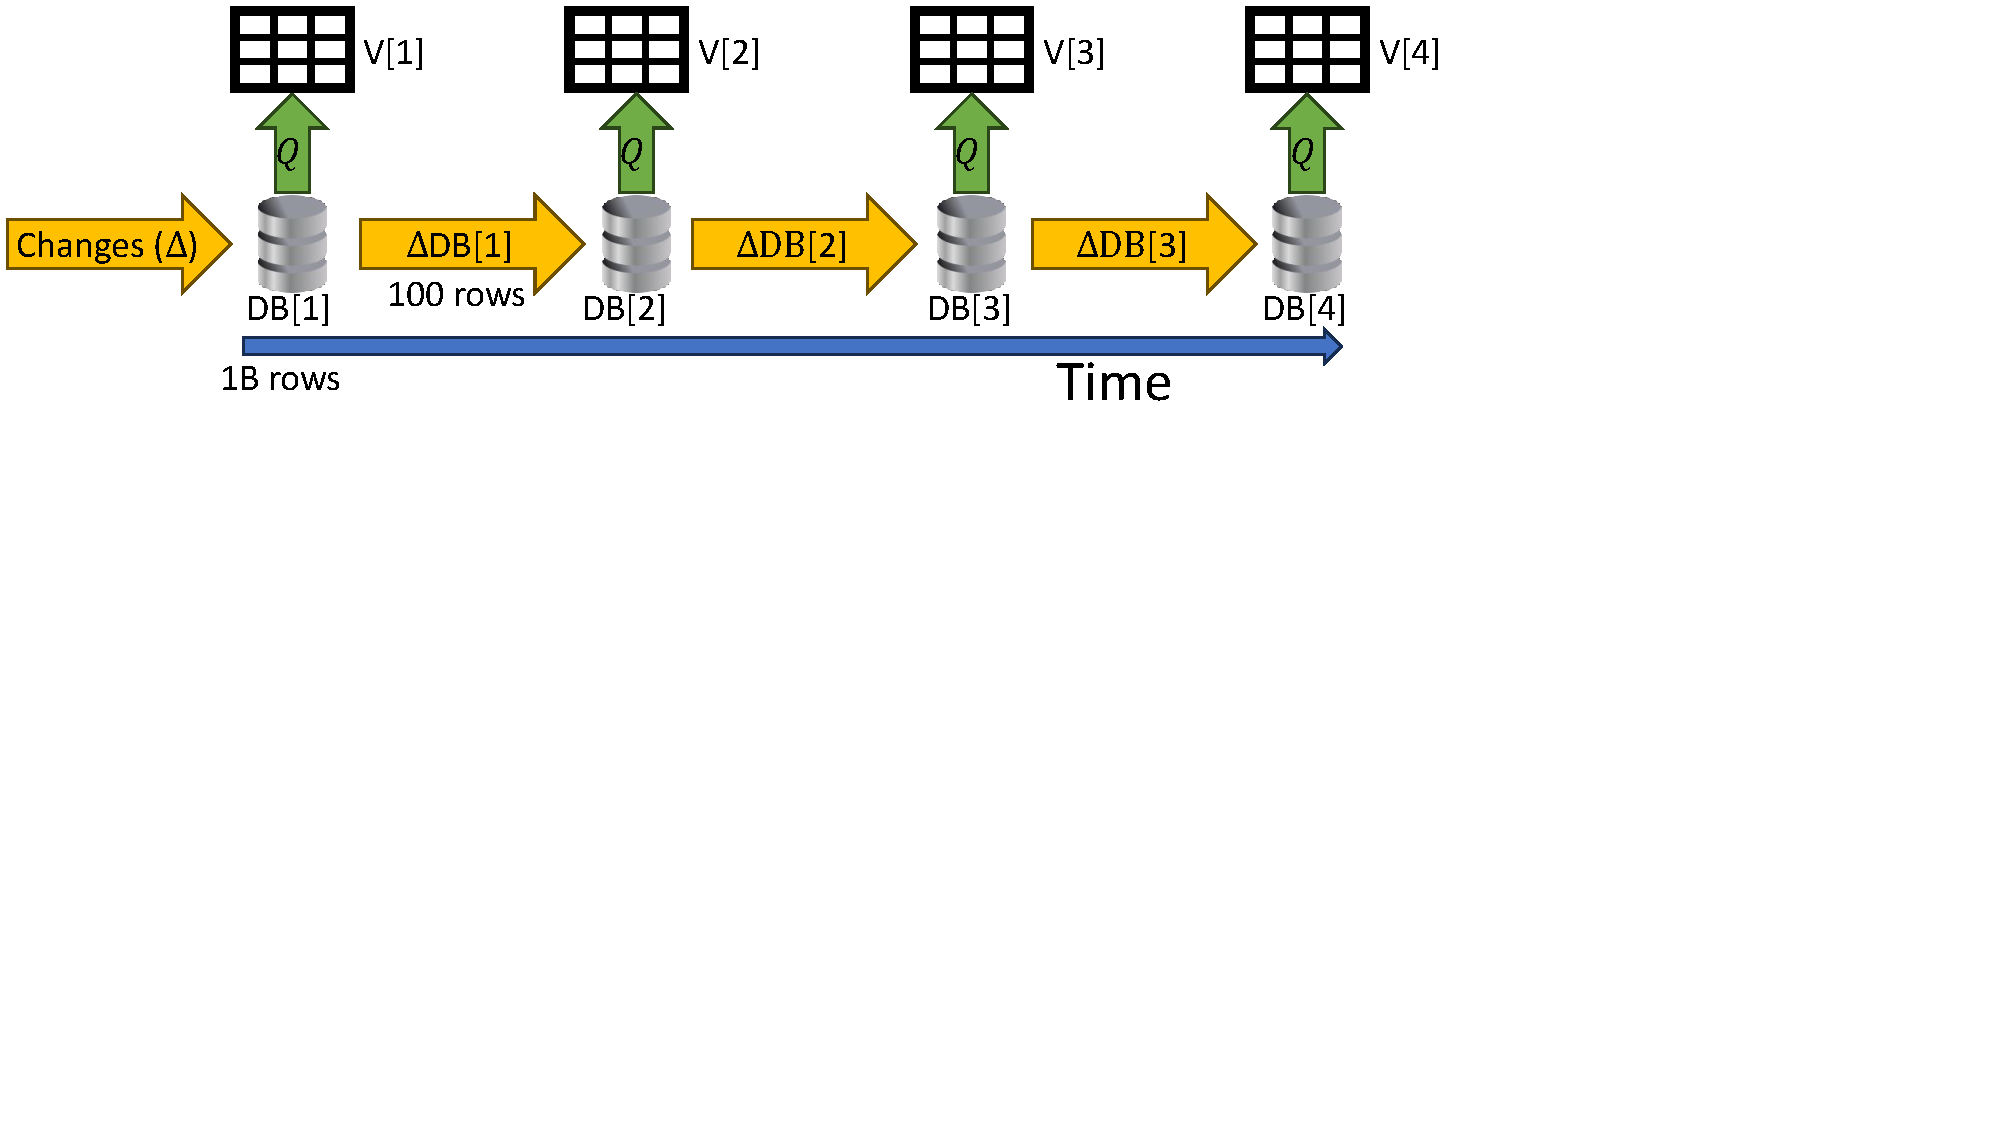
\includegraphics[trim={0 3.9in 4.1in 0},clip,scale=.30]{view.pdf}

The naive solution is expensive.  After the first version of the view
has been constructed, an ideal algorithm would compute only
\emph{changes} to the view $\Delta V$ by performing work proportional
to $O(|\Delta DB|)$.  Ideally, we want to construct a new query
$\inc{Q}$ with the property that $\Delta V = \inc{Q}(\Delta DB)$,
i.e., $\inc{Q}$ can compute the change of the view from the change of
the database:

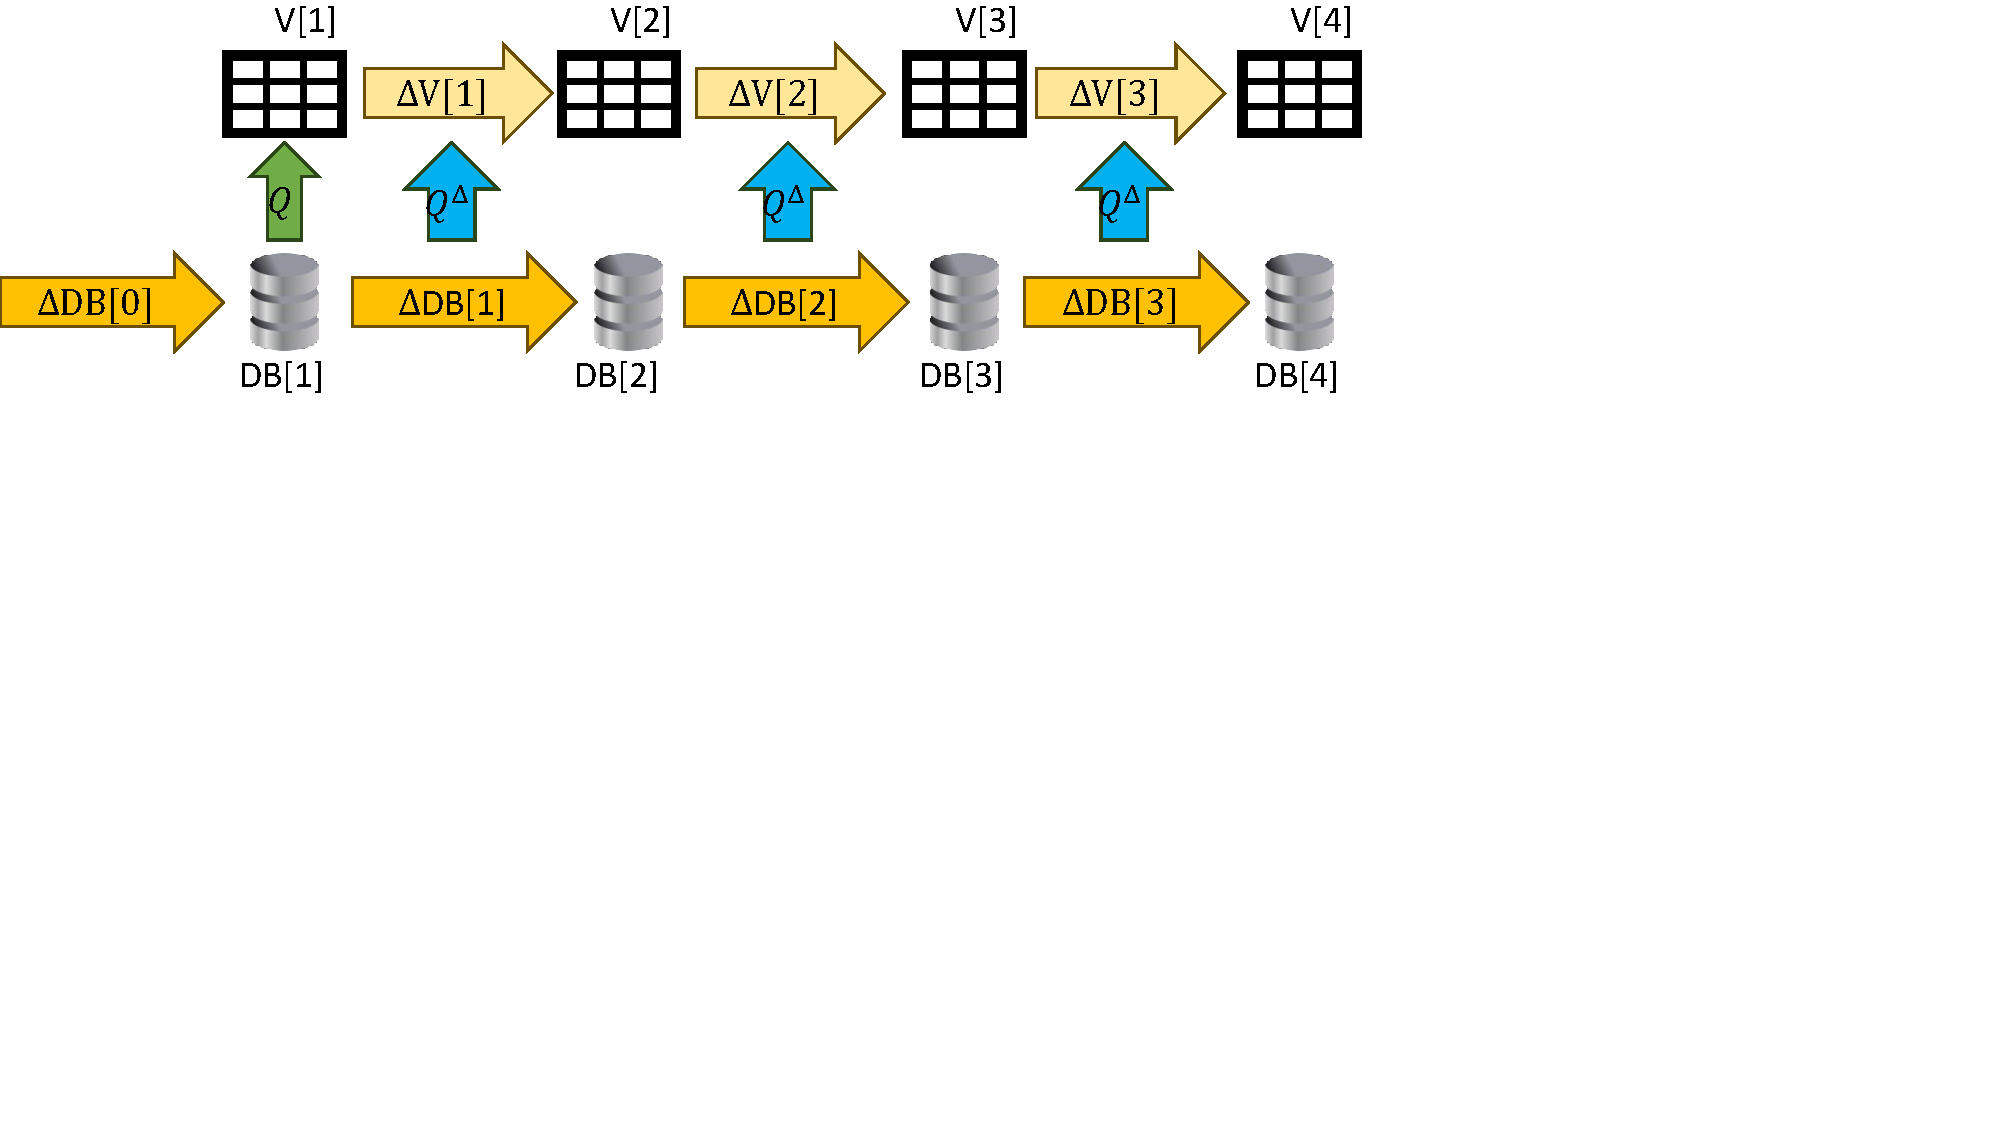
\includegraphics[trim={0 4.5in 4.1in 0},clip,scale=.30]{incview.pdf}

We call $\inc{Q}$ the \emph{incremental} version of $Q$.  If one
thinks of $\inc{Q}$ as a function of a database change, one can show
that the ideal solution as described above is impossible to reach.

In this paper we provide a new perspective, by proposing a new way to
precisely define $\inc{Q}$ as a form of \emph{computation on streams}.
Our model is inspired by Digital Signal Processing
DSP~\cite{rabiner-book75}, applied to databases, hence the name \dbsp.
$\inc{Q}$ can be very efficient.  As for traditional database queries,
the performance of $\inc{Q}$ depends both on the query $Q$ but also on
the actual data that the query is applied to.  While one cannot give a
simple closed form for the speed-up obtained by $\inc{Q}$, as a rule
of thumb, for essentially all practical queries $Q$, the incremental
version of $\inc{Q}$ that our algorithm constructs, is faster than $Q$
by a factor of $O(|DB| / |\Delta DB|)$.  In practice this may be an
improvement of several orders of magnitude.  For our example above
$|DB| \approx 10^9$ and $|\Delta DB| \approx 10^2$, this makes
$\inc{Q}$ \textbf{10 million times} faster than $Q$!

Instead of treating the database as a monolithic changing object, we
treat it as a \emph{sequence} or \emph{stream} of database snapshots.
Similarly, the view snapshots form a stream.  \dbsp is a simple
programming language for computing on streams; the inputs and outputs
of \dbsp programs are streams of arbitrary values.

%Whereas previous IVM solutions are based on defining a notion of a
%(partial) derivative of $Q$ with respect to its inputs, our definition
%only requires computing \emph{derivatives of streams} as functions of
%time.  Derivatives of streams are always well-defined if the data
%computed on has a notion of difference that satisfies some simple
%mathematical properties --- specifically, that it forms a commutative
%group.  (Fortunately, relational databases can be modeled in such a
%way~\cite{green-pods07, koch-pods10}.)

The \dbsp language has only 4 operators.  However, it can express a
rich set of computations on streams, including repeated computations
(similar to the repeated queries $Q$ above), recursive computations
that compute fixed points (as done by Datalog programs), streaming
computations, and incremental computations (which we define shortly).
The full paper~\cite{budiu-vldb23} gives a precise mathematical
description of \dbsp, this presentation is simplified to convey the
main intuitions behind the design.  We omit the related work section
from this presentation.

The central result of this paper is Algorithm~\ref{algorithm-inc}
which, given a \dbsp program that computes on a stream of values,
mechanically transforms it into an incremental \dbsp program that
computes on a stream of changes.

\dbsp is not tied to databases in any way; it is in fact a
Turing-complete language that can be used for many other purposes.
But it works particularly well in the area of databases, for two
reasons:

\begin{itemize}
  \item \dbsp operates on values that must form a commutative group.
    Databases can be modeled as values from a commutative group.
  \item \dbsp reduces the problem of incrementalizing a complex
    program to the problem of incrementalizing each primitive
    operation that appears in the program.  For the domain of
    databases there are known efficient incremental implementations
    for all primitive operations.
\end{itemize}

%\dbsp has several attractive properties:
%
%\begin{enumerate}
%\item it is \textbf{simple}.  \dbsp has only 4 operators, and it is
%  built entirely on elementary concepts such as functions and
%  algebraic groups.
%\item it is \textbf{expressive}.  It can be used to define precisely
%  multiple concepts: traditional queries, streaming computations, and
%  incremental computations.
%\item mathematically \textbf{precise}.  All the results in this paper
%  have been formalized and checked using the Lean proof
%  assistant~\cite{moura-cade15}.
%\item it is \textbf{modular}, in the following two ways:
%(a) the incremental version of a complex query can be reduced
%recursively to incrementalizing its component subqueries.
%This gives a simple, syntactic,
%heuristic-free algorithm (Algorithm~\ref{algorithm-inc})
%that converts an arbitrary \dbsp query plan to its incremental form.
%(b) Extending \dbsp to support new primitive operators is easy,
%and they immediately benefit from the rest of the theory of
%incrementalization.
%An important consequence of modularity is that the theory
%can be efficiently implemented, as we
%briefly discuss in \refsec{sec:implementation}.
%\end{enumerate}

\subsection{Circuits and Streams}\label{sec:intro-circuits}

In this paper we use circuit diagrams to depict programs.  In a
circuit a rectangle represents a function, and an arrow represents an
input or output value.  The following diagram shows a function $f$
consuming two inputs $i$ (input 0) and $j$ (input 1) and producing one
output $o = f(i, j)$:
%
\begin{center}
\begin{tikzpicture}[auto,>=latex,inner sep=0mm]
  \node[block, minimum height=.7cm, minimum width=.5cm] (function) {$f$};
  \node[below=1mm of function.north west,font=\tiny,anchor=north west] (0) {0};
  \node[above=1mm of function.south west,font=\tiny,anchor=south west] (1) {1};
  \node[left of=0, node distance=.5cm] (input0) {$i$};
  \node[left of=1, node distance=.5cm] (input1) {$j$};
  \node[right of=function, node distance=.8cm] (output) {$o$};
  \draw[->] (input0) -- (0);
  \draw[->] (input1) -- (1);
  \draw[->] (function) -- (output);
\end{tikzpicture}
\end{center}
%
Most of the functions we deal with are commutative, and in this case
we do not need to label the inputs.  We also avoid showing input
labels if the arrows are labeled in the text and can be used to
distinguish the order of inputs; thus we will display the circuit
above as:
%
\begin{center}
  \begin{tikzpicture}[auto,>=latex, node distance=.7cm]
    \node[] (input0) {$i$};
    \node[below of=input0,node distance=.2cm] (dummy) {};
    \node[below of=dummy,node distance=.2cm] (input1) {$j$};
    \node[block, right of=dummy] (T) {$f$};
    \node[right of=T] (output) {$s$};
    \draw[->] (input0) -- (T);
    \draw[->] (input1) -- (T);
    \draw[->] (T) -- (output);
  \end{tikzpicture}
\end{center}
%
Functions, and their circuits, can be composed, as in the following
example for the function $o = g(s) + (f(s) \times s)$:
%
\begin{center}
\begin{tikzpicture}[auto,>=latex]
  \node[] (input) {$s$};
  \node[] [right of=input, node distance=.4cm] (dummy) {};
  \node[block, below of=dummy, node distance=.7cm] (S1) {$f$};
  \node[block, right of=S1] (T1) {$\times$};
  \node[block, right of=T1] (T2) {$+$};
  \node[block, above of=T2, node distance=.7cm] (S2) {$g$};
  \node[right of=T2, node distance=.7cm] (output) {$o$};
  \draw[->] (input) -| (S1);
  \draw[->] (input) -| (T1);
  \draw[->] (S1) -- (T1);
  \draw[->] (T1) -- (T2);
  \draw[->] (input) -- (S2);
  \draw[->] (T2) -- (output);
  \draw[->] (S2) -- (T2);
\end{tikzpicture}
\end{center}
%
We say that two circuits are \defined{equivalent} if they compute the
same function.  We use the symbol $\cong$ to indicate circuit
equivalence.  For example, we have the following circuit equivalence
(where $\circ$ is function composition):

\noindent
\begin{tabular}{m{3cm}m{.3cm}m{3cm}c}
\begin{tikzpicture}[auto,>=latex]
  \node[] (input) {$s$};
  \node[block, right of=input] (g) {$g$};
  \node[block, right of=g] (f) {$f$};
  \node[right of=f] (output) {$o$};
  \draw[->] (input) -- (g);
  \draw[->] (g) -- (f);
  \draw[->] (f) -- (output);
\end{tikzpicture}
&
$\cong$
&
\begin{tikzpicture}[auto,>=latex]
    \node[] (input) {$s$};
    \node[block, right of=input, node distance=1cm] (fg) {$f \circ g$};
    \node[right of=fg, node distance=1cm] (output) {$o$};
    \draw[->] (input) -- (fg);
    \draw[->] (fg) -- (output);
\end{tikzpicture}
&
(*)
\end{tabular}

\subsection{Streams}

The core notion of \dbsp is the \textbf{stream}.  Given a set $A$, a
\defined{stream} \emph{of values from $A$} is an infinite sequence of
values from $A$.  $\stream{A}$ denotes the set of all streams with
values from $A$.  We write $s[t]$ for the $t$-th element of the stream
$s$.  Think of $t$ as the ``time'' and of $s[t]\in A$ as the value of
the stream $s$ ``at time'' $t$.  In examples we show streams as a
sequence of boxes, where time goes from \emph{right to left}: e.g.,
the stream $s[t] = t$ is:

\begin{center}
\begin{tabular}{cc}
  \sv{0 1 2 3 4} \\
  $\xleftarrow[\hspace{1cm}\mathrm{time}\hspace{1cm}]{}$
\end{tabular}
\end{center}

%\begin{definition}[stream operator]
A \defined{stream operator} is a function that computes on streams and
produces streams.
%\end{definition}
In general we use ``operator'' for streams, and ``function'' for
computations on ``scalar'' values.

To make figures easier to interpret, we use arrows with a double head
to depict streams.  Note that this notation differs from the one in
the original paper~\cite{budiu-vldb23}, where we used single arrows
for streams in most cases.  The following diagram shows a stream
operator $T$ consuming two input streams $s_0$ and $s_1$ and producing
one output stream $s$:

\begin{center}
\begin{tikzpicture}[auto,>=latex,inner sep=0mm]
  \node[block, minimum height=.7cm, minimum width=.5cm] (function) {$T$};
  \node[below=1mm of function.north west,font=\tiny,anchor=north west] (0) {0};
  \node[above=1mm of function.south west,font=\tiny,anchor=south west] (1) {1};
  \node[left of=0, node distance=0.8cm] (input0) {$s_0$};
  \node[left of=1, node distance=0.8cm] (input1) {$s_1$};
  \node[right of=function, node distance=.8cm] (output) {$s$};
  \draw[->>] (input0) -- (0);
  \draw[->>] (input1) -- (1);
  \draw[->>] (function) -- (output);
\end{tikzpicture}
\end{center}

We write $s = T(s_0, s_1)$.
%\begin{definition}(lifting)
Given a function $f: A \to B$, we define a stream operator $\lift{f}
:\stream{A} \to \stream{B}$ (read as ``$f$ lifted'') by applying
function $f$ to the input stream(s) independently at each point in
time:
\begin{center}
  \begin{tikzpicture}[auto,>=latex]
    \node[] (input) {$\sv{a b c d e}$};
    \node[block, right of=input, node distance=2.2cm] (f) {$\lift{f}$};
    \node[right of=f, node distance=2.8cm] (output) {$\sv{f(a) f(b) f(c) f(d) f(e)}$};
    \draw[->>] (input) -- (f);
    \draw[->>] (f) -- (output);
  \end{tikzpicture}
\end{center}
%\end{definition}

To simplify the notation, we will write $a + b$ for streams $a, b$
instead of $a (\lift{+}) b$; we will also write $-a$ instead of
$(\lift{-})a$.

\subsection{Databases as streams}

We generally think of streams as sequences of ``small'' values, such
as insertions or deletions in a database.  However, we also treat the
whole database as a \emph{stream of database snapshots}.  We model a
database as a stream $DB$.  Time is not wall-clock time, but counts
the transactions applied to the database.  Since transactions are
linearizable, they have a total order.  $DB[t]$ is the snapshot of the
database contents after $t$ transactions have been applied.  This
notation is apparent in the diagrams in \refsec{sec:intro-incremental}.

Database transactions also form a stream $\Delta DB$, this time a
stream of \emph{changes}, or \emph{deltas}, that are applied to the
database.  The values of this stream are defined by $(\Delta DB)[t] =
DB[t] - DB[t-1]$, where ``$-$'' stands for the difference between two
databases, a notion that we will soon make more precise.  The $\Delta
DB$ stream can be produced from the $DB$ stream by the \emph{stream
differentiation} operator $\D$; this operator produces as its output
the stream of changes from its input stream; we have thus $\D(DB) =
\Delta DB$.

Conversely, the database snapshot at time $t$ is the cumulative result
of applying all transactions up to $t$: $DB[t] = \Delta DB[0] + \Delta
DB[1] + \ldots + \Delta DB[t]$.  The stream operator $\I$ is defined
to produce an output by adding up all previous inputs.  We call this
operator \emph{stream integration}, the inverse of differentiation.
The following diagram shows the relationship between the streams
$\Delta DB$ and $DB$:
\begin{center}
\begin{tikzpicture}[auto,>=latex,minimum width=.5cm, node distance=1.2cm]
  \node[] (input) {$\Delta DB$};
  \node[block, right of=input] (I) {$\I$};
  \node[right of=I] (output) {$DB$};
  \node[block, right of=output] (D) {$\D$};
  \node[right of=D] (end) {$\Delta DB$};
  \draw[->>] (input) -- (I);
  \draw[->>] (I) -- (output);
  \draw[->>] (output) -- (D);
  \draw[->>] (D) -- (end);
\end{tikzpicture}
\end{center}

What is a view in our streaming model?  It is also a stream!  Suppose
we are given a query $Q$ defining a view $V$.  For each snapshot of
the database stream we have a snapshot of the view: $V[t] = Q(DB[t])$.
A view is thus just a lifted query: $V = (\lift{Q})(DB)$.

Armed with these basic definitions, we can precisely define IVM.  What
does it mean to maintain a view incrementally?  A maintenance
algorithm needs to compute the \emph{changes} to the view given the
changes to the database. Given a query $Q$, a key contribution of this
paper is the definition of its \emph{incremental version} $\inc{Q}$,
using stream integration and differentiation, depicted graphically as:
%
\begin{center}
\begin{tikzpicture}[auto,>=latex,minimum width=.5cm]
  \node[] (input) {$\Delta DB$};
  \node[block, right of=input, node distance=1.3cm] (I) {$\I$};
  \node[block, right of=I, node distance=1.3cm] (Q) {$\lift{Q}$};
  \node[block, right of=Q, node distance=1.3cm] (D) {$\D$};
  \node[right of=D] (output) {$\Delta V$};
  \draw[->>] (input) -- (I);
  \draw[->>] (I) -- node (db) {$DB$} (Q);
  \draw[->>] (Q) -- node (B) {$V$} (D);
  \draw[->>] (D) -- (output);
  \draw[decorate, decoration = {brace, raise=13pt}] (input) -- (output)
  node[pos=.5, above=13pt]{$\inc{Q}$};
\end{tikzpicture}
\end{center}
%
Mathematically this is written as $\inc{Q} = \D \circ (\lift{Q}) \circ
\I$.  The incremental version of a query $Q$ is a \emph{streaming
operator} $\inc{Q}$ which computes directly on changes and produces
changes.  The incremental version of a query is thus always
well-defined.  The above definition gives us one way to compute a
query incrementally, but applying it naively produces an inefficient
execution, since it reconstructs the database at each step.  It is in
fact as bad as the naive solution.  In \refsec{sec:incremental} we
show how we can optimize the implementation of $\inc{Q}$. The key
property is that the incremental composition of two queries $Q_1$ and
$Q_2$ is the composition of their incremental versions: $\inc{(Q_1
  \circ Q_2)} = \inc{Q_1} \circ \inc{Q_2}$.

Armed with this general theory of incremental computation, in
\secref{sec:relational} we show how to model relational queries in
\dbsp.  This immediately gives us a general algorithm to compute the
incremental version of any relational query.  These results were
previously known, but they are cleanly modeled by \dbsp.
\secref{sec:recursion} shows how programs containing recursion can be
implemented and incrementalized in \dbsp.  For example, given an
implementation of transitive closure in the natural recursive way, our
algorithm produces a program that efficiently maintains the transitive
closure of a graph as nodes and edges are added and deleted.

\subsection{Contributions}

This work makes the following contributions:
\begin{enumerate}
  \item We introduce \dbsp, a simple but expressive language for
    streaming computation. \dbsp gives an elegant formal foundation
    unifying the manipulation of streaming and incremental
    computations.
  \item An algorithm for incrementalizing any streaming
    computation expressed in \dbsp in the presence of arbitrary
    insertions and deletions from any of the data sources.
  \item An illustration of how \dbsp can model various classes of
    practical queries, such as relational algebra, nested relations,
    aggregations, and Datalog.
  \item The first general and machine-checked theory of IVM.  All the
    theoretical results in the original version of this
    paper~\cite{budiu-vldb23} have been checked~\cite{dbsp-theory}
    using the Lean proof assistant~\cite{moura-cade15}.
  \item A practical open-source implementation of this theory as a
    runtime and a SQL compiler.
\end{enumerate}

